\section{Background Estimation}
\label{sec:background}

The general approach for background estimation is to derive data/MC scale factor corrections from background enriched control regions (CR) and apply these to the MC predictions for the signal region (SR). Formally, for a particular background process,
\begin{equation}
  N_{\mbox{\scriptsize{SR}}}^{\mbox{\scriptsize{predict}}} = N_{\mbox{\scriptsize{SR}}}^{\mbox{\scriptsize{MC}}}
\left(\frac{N_{\mbox{\scriptsize{CR}}}^{\mbox{\scriptsize{data}}}}{N_{\mbox{\scriptsize{CR}}}^{\mbox{\scriptsize{MC}}}}\right),
\end{equation}
where $N_{\mbox{\scriptsize{SR}}}^{\mbox{\scriptsize{predict}}}$ is the signal region prediction for the background of interest, $N_{\mbox{\scriptsize{SR}}}^{\mbox{\scriptsize{MC}}}$ is the MC yield in the signal region, and $N_{\mbox{\scriptsize{CR}}}^{\mbox{\scriptsize{data}}}$ and $N_{\mbox{\scriptsize{CR}}}^{\mbox{\scriptsize{MC}}}$ are the yields in the control region for data and MC respectively. For a cut-and-count analysis, the formula states the MC yields in the SR are corrected by the ratio of data-to-MC yields in the CR. For a shape analysis, the formula implies bin-by-bin correction factors in the variable used for signal extraction (i.e. $\met$).

To handle signal contamination in the control regions and as well as backgrounds that contribute substantially to multiple control regions, the signal extraction and scale factor derivation will be performed simultaneously across all signal and control regions. (This is not yet done for this note.)

\subsection{Backgrounds: Hadronic channel}
\label{subsec:bkg_hadronic}

The main backgrounds in this channel are semileptonic $\ttbar$, $\Wjets$, and $\Z(\Nu\Nu)+$jets, and control regions enriched in these backgrounds are defined in the following. Also, a control region for QCD is defined to validate that the background is expected to be small.

\subsubsection{Control region for \texorpdfstring{$\ttbar$}{ttbar}}
\label{subsubsec:bkg_hadronic_ttbar}

A control region enriched in semileptonic $\ttbar$ can be obtained by requiring exactly one ``Tight'' electron or muon with $M_T<160\:\GeV$, while keeping all other selection requirements.\iffalse For the categories with boosted top tags, the subjet $\Bot$-tag requirements are dropped.To obtain a $\met$ template, the four-momentum of the lepton is removed and it is this lepton subtracted $\met$ quantity that must be greater than $250\:\GeV$.\fi From the studies shown in Appendix ~\ref{app:CR}, we determine that removal of the lepton four-momentum from the $\met$ in this control region isn't necessary in order to model the $\met$ distribution in the signal region. The yields are listed in Table~\ref{tab:hadronic_bkg_tt1l_yields}. The \iffalse lepton subtracted \fi $\met$ distributions in the control region for the inclusive selection is shown in Fig.~\ref{fig:incl_hadronic_1l_fmet} for both the electron and muon selection. 

\begin{table}[!ht]
\centering
\begin{tabular}{|c|r|r|}
\hline
  Process & \multicolumn{1}{|c|}{Electron Channel} & \multicolumn{1}{|c|}{Muon Channel} \\
\hline
  Diboson         & $   1.09 \pm  0.33$ & $  0.97 \pm  0.27$ \\
  \Zjets            & $ 0.58 \pm  0.22$ &$4.07 \pm  1.23$ \\
  Single \Top    & $ 52.12 \pm 1.48$ &  $57.99 \pm  1.51$ \\
  \Wjets            & $   34.97 \pm  1.10$ & $  46.53 \pm  1.53$ \\
  $\ttbar$   & $   618.07 \pm  3.17$ & $  710.05 \pm  3.30$ \\
  QCD        & $ 0.00 \pm 0.00$ & $0.00\pm  0.00$ \\
\hline
SM expected     & $706.83 \pm 3.69$ & $819.61 \pm 4.14$ \\
 \hline
  Observed        & $719.00 \pm 0.00$ & $883.00 \pm 0.00$ \\
\hline
  $M_\chi=1\:\GeV\:, M_\phi=10\:\GeV\:$       & $  1.30 \pm  0.12$ &  $2.30  \pm  0.16$ \\
\hline
\end{tabular}
\caption{Expected and observed yields for $1.3\:\ifb$ in the $\ttbar$ control region for the hadronic channel.}
\label{tab:hadronic_bkg_tt1l_yields}
\end{table}

\begin{figure}[htbp]
  \centering
  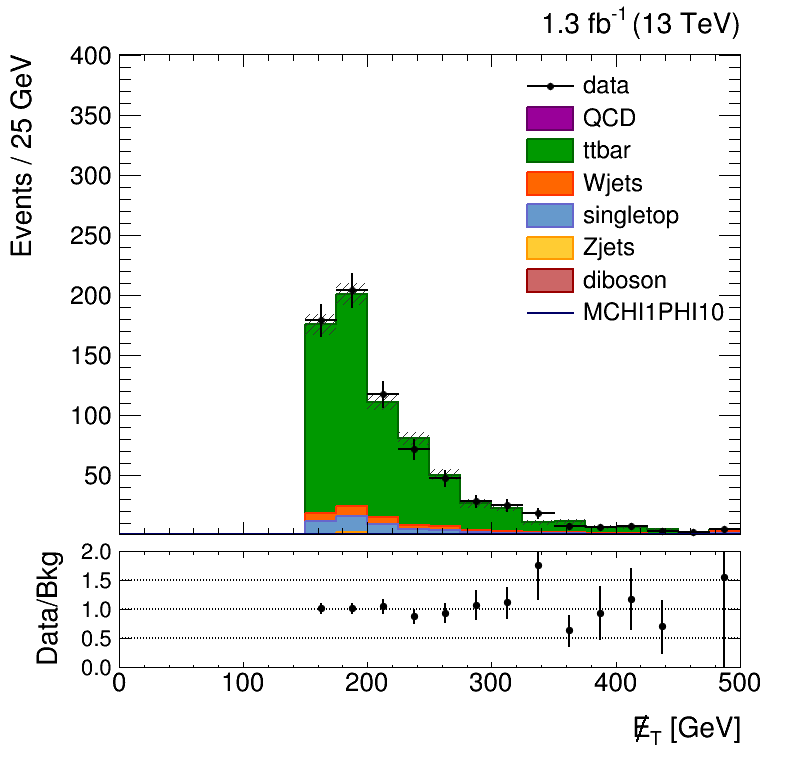
\includegraphics[width=0.48\textwidth]{figures/hMETlinear_CRttbar_el.png}
  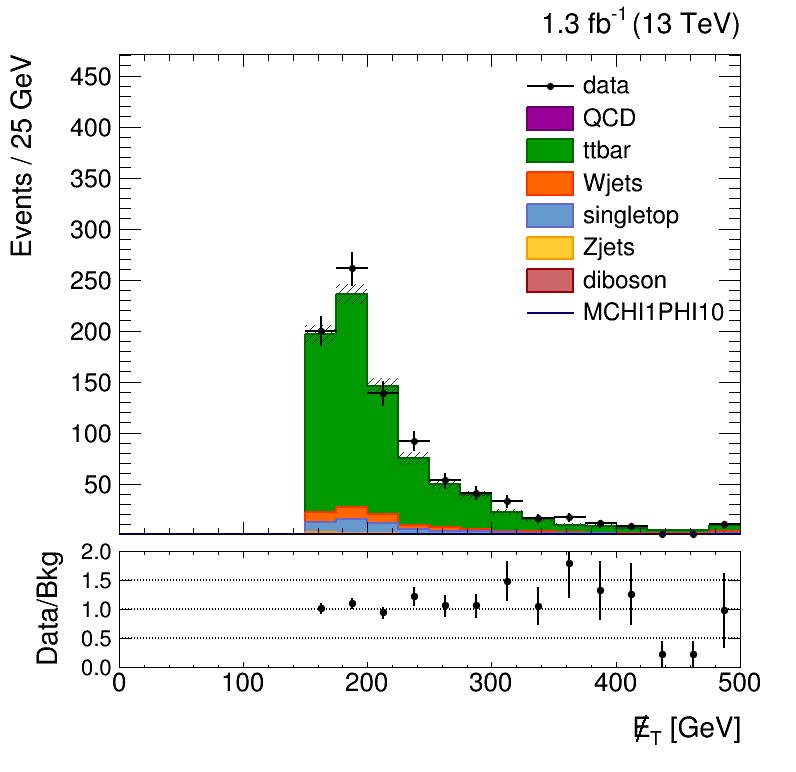
\includegraphics[width=0.48\textwidth]{figures/hMETlinear_CRttbar_mu.png}
    \caption{The $\met$ distribution in the $\ttbar$ control region with electron (left) and muon (right) selection for the hadronic channel.}
  \label{fig:incl_hadronic_1l_fmet}
\end{figure}

\clearpage
\subsubsection{Control region for \texorpdfstring{$V+$jets}{Vjets}}
\label{subsubsec:bkg_hadronic_vjets}

By requiring no $\Bot$-tagged jets in the event and keeping all other cuts the same, a sample enriched in $\Wjets$ and $\Z(\Nu\Nu)+$jets can be obtained. From the studies shown in Appendix ~\ref{app:CR}, we determine that removal of the lepton four-momentum from the $\met$ in the $V+$jets control region isn't necessary in order to model the $\met$ distribution in the signal region. \iffalse For the categories with boosted top tags, the subjet $\Bot$-tag requirements are dropped.\fi  The yields are listed in Table~\ref{tab:hadronic_bkg_vjets_yields}. The $\met$ distributions in the control region for the inclusive selection is shown in Fig.~\ref{fig:incl_hadronic_0b_met}.

\begin{table}[!ht]
\centering
\begin{tabular}{|c|r|}
\hline
  Process & \\
\hline
  Diboson         & $ 33.10 \pm 1.89 $ \\
  \Zjets            & $681.22 \pm 3.91$ \\
  Single \Top    & $21.65 \pm 0.95 $ \\
  \Wjets            & $ 1341.57 \pm 11.81 $ \\
  $\ttbar$   & $    221.19 \pm 1.94$ \\
  QCD        & $ 19.54 \pm 2.96$ \\
\hline
SM expected     & $  2318.28 \pm 13.11$\\
 \hline
  Observed        & $2380.00 \pm 0.00$ \\
\hline
  $M_\chi=1\:\GeV\:, M_\phi=10\:\GeV\:$       & $ 2.76 \pm 0.18$ \\
\hline
\end{tabular}
\caption{Expected yields for $1.3\:\ifb$ in the $V+$jets control region for the hadronic channel.}
\label{tab:hadronic_bkg_vjets_yields}
\end{table}

\begin{figure}[htbp]
  \centering
  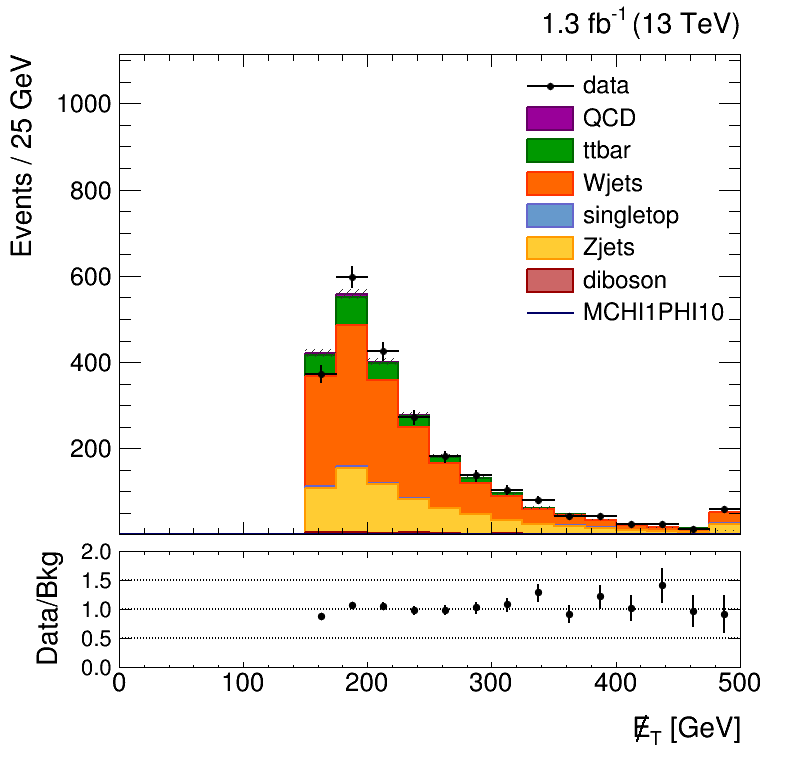
\includegraphics[width=0.48\textwidth]{figures/hMETlinear_CRvjets_0b.png}
  \caption{The $\met$ distribution in the $V+$jets control region for the hadronic channel.}
  \label{fig:incl_hadronic_0b_met}
\end{figure}

\subsubsection{Control region for \texorpdfstring{$\Wjets$}{Wjets}}
\label{subsubsec:bkg_hadronic_wjets}

A control region enriched in $\Wjets$ can be obtained by requiring a ``Tight'' electron or muon and no $\Bot$-tagged jets, while keeping all other selection requirements. \iffalse For the categories with boosted top tags, the subjet $\Bot$-tag requirements are dropped. \fi To obtain a $\met$ template, we do not remove the lepton four-momentum and require that this $\met$ quantity that must be greater than $250\:\GeV$. Studies that support retaining the lepton \pt\: are detailed in Appendix~\ref{app:CR}.The expected and observed yields are listed in Table~\ref{tab:hadronic_bkg_vjets_yields}. The \iffalse lepton subtracted \fi $\met$ distributions in the control region for the inclusive selection is shown in Fig.~\ref{fig:incl_hadronic_1l0b_fmet} for both the electron and muon selection.

\begin{table}[!ht]
\centering
\begin{tabular}{|c|r|r|}
\hline
  Process & \multicolumn{1}{|c|}{Electron Channel} & \multicolumn{1}{|c|}{Muon Channel} \\
\hline
  Diboson         & $  000000$ & $17.72 \pm 1.48$ \\
  \Zjets            & $20.61 \pm1.98$ &  $24.65 \pm 2.07$ \\
  Single \Top    & $ 23.65 \pm 0.98$ &  $30.23 \pm 1.13$ \\
  \Wjets            & $ 770.08 \pm 6.72$ & $  886.25 \pm 7.32$ \\
  $\ttbar$   & $   253.06 \pm 2.03$ & $  313.48 \pm 2.30$ \\
  QCD        & $ 3.13 \pm 1.32$ & $0.64 \pm 0.60$ \\
\hline
SM expected     & $1088.29 \pm 7.62$ & $1272.98 \pm 8.19$ \\
 \hline
  Observed        & $939.00 \pm 0.00$ & $1167.00 \pm 0.00$ \\
\hline
  $M_\chi=1\:\GeV\:, M_\phi=10\:\GeV\:$       & $  0.94 \pm  0.10$ &  $1.19  \pm  0.12$ \\
\hline
\end{tabular}
\caption{Expected and observed yields for $1.3\:\ifb$ in the $\Wjets$ control region for the hadronic channel.}
\label{tab:hadronic_bkg_wjets_yields}
\end{table}

\begin{figure}[htbp]
  \centering
  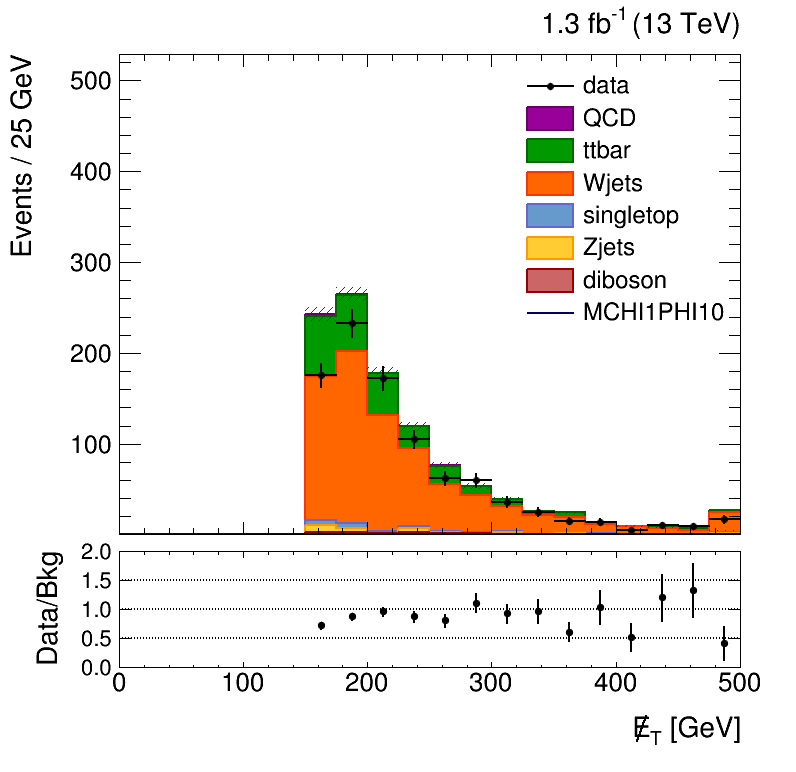
\includegraphics[width=0.48\textwidth]{figures/hMETlinear_CRwjets_el.png}
  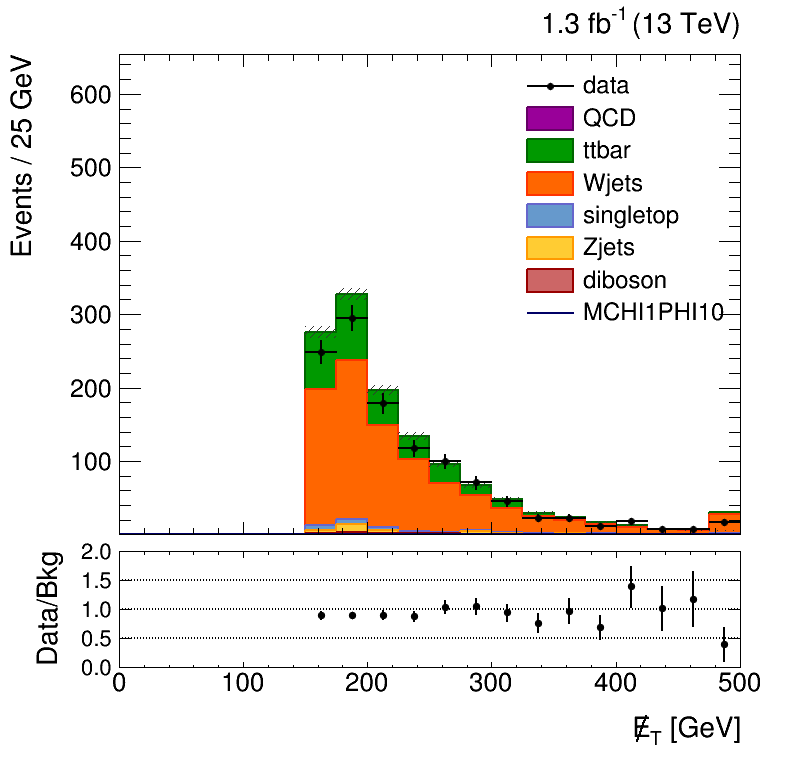
\includegraphics[width=0.48\textwidth]{figures/hMETlinear_CRwjets_mu.png}
  \caption{The $\met$ distribution in the $\Wjets$ control region for the hadronic channel for electron (left) and muon (right) selection.}
  \label{fig:incl_hadronic_1l0b_fmet}
\end{figure}


%2j/0b
%  *     Z+jets    954.88 +/-   6.92
%  *   single t    332.13 +/-   6.67
%  *     W+jets  42025.86 +/- 136.36
%  * t#bar{t}+V      0.75 +/-   0.10
%  * t#bar{t}(had)      0.16 +/-   0.16
%  * t#bar{t}(2l)    122.08 +/-   4.47
%  * t#bar{t}(1l)    639.34 +/-  10.22
%  ============
%     total bkg  44075.21 +/- 137.16
%      DM 1 GeV      3.41 +/-   0.37

%2j/2b
%  *     Z+jets      2.46 +/-   0.31
%  *   single t     31.57 +/-   2.11
%  *     W+jets     77.21 +/-   5.23
%  * t#bar{t}+V      0.11 +/-   0.04
%  * t#bar{t}(had)      0.00 +/-   0.00
%  * t#bar{t}(2l)     26.80 +/-   2.09
%  * t#bar{t}(1l)     71.75 +/-   3.42
%  ============
%     total bkg    209.91 +/-   6.93
%      DM 1 GeV      0.90 +/-   0.19


%2j/1b
%  *     Z+jets     78.01 +/-   1.91
%  *   single t    293.13 +/-   6.49
%  *     W+jets   3057.11 +/-  35.02
%  * t#bar{t}+V      1.07 +/-   0.12
%  * t#bar{t}(had)      0.00 +/-   0.00
%  * t#bar{t}(2l)    190.56 +/-   5.58
%  * t#bar{t}(1l)    700.46 +/-  10.70
%  ============
%     total bkg   4320.34 +/-  37.65
%      DM 1 GeV      6.13 +/-   0.50

\clearpage
\subsubsection{Control region for \texorpdfstring{$\Zjets$}{Zjets}}
\label{subsubsec:bkg_hadronic_zjets}

A control region enriched in $\Zjets$ can be obtained by requiring a pair of ``Tight'' electrons or muons, with dilepton mass between $60\:\GeV$ and $120\:\GeV$, and no $\Bot$-tagged jets, while keeping all other selection requirements. The agreement between the $\met$ distribution in the $\Zjets$ control and signal regions shown in Appendix~\ref{app:CR} validate the following extracted $\met$ distribution. \iffalse For the categories with boosted top tags, the subjet $\Bot$-tag requirements are dropped. \fi To obtain a $\met$ template for $\Z\To\Nu\Nu$, the four-momentum of the dilepton system is removed and it is the dilepton subtracted $\met$ that must be greater than $250\:\GeV$. The yields are listed in Table~\ref{tab:hadronic_bkg_zjets_yields}. The lepton subtracted $\met$ distributions in the control region for the inclusive selection is shown in Fig.~\ref{fig:incl_hadronic_2l0b_fmet}.

\begin{table}[!ht]
\centering
\begin{tabular}{|c|r|r|}
\hline
  Process & \multicolumn{1}{|c|}{$ee$} & \multicolumn{1}{|c|}{$\mu\mu$} \\
\hline
  Diboson         & $  3.70 \pm 0.47$ & $4.15 \pm 0.46$ \\
  \Zjets            & $134.70 \pm 4.50$ &  $213.82 \pm 5.85$ \\
  Single \Top    & $ 0.83 \pm 0.18$ &  $0.79 \pm 0.17$ \\
  \Wjets            & $ 0.35 \pm 0.12$ & $  0.21 \pm 0.11$ \\
  $\ttbar$   & $   10.52 \pm 0.41$ & $   16.72 \pm 0.53$ \\
  QCD        & $0.07 \pm 0.07$ & $ 1.63 \pm 1.08$ \\
\hline
SM expected     & $150.17 \pm 4.55$ & $237.33 \pm 5.99$ \\
 \hline
  Observed        & $170.00 \pm 0.00$ & $274.00 \pm 0.00$ \\
\hline
  $M_\chi=1\:\GeV\:, M_\phi=10\:\GeV\:$       & $  0.00 \pm 0.00$ &  $0.02 \pm 0.02$ \\
\hline
\end{tabular}

\caption{Expected yields for $1.3\:\ifb$ in the $\Zjets$ control region with dileptons for the hadronic channel.}
\label{tab:hadronic_bkg_zjets_yields}
\end{table}

\begin{figure}[htbp]
  \centering
  \includegraphics[width=0.48\textwidth]{figures/hMETNoLepLinear_CRzjets_el.png}
  \includegraphics[width=0.48\textwidth]{figures//hMETNoLepLinear_CRzjets_mu.png}
  \caption{The $\met$ distribution in the $\Zjets$ control region with dileptons for the hadronic channel with the double electron (left) and double muon (right) selection.}
  \label{fig:incl_hadronic_2l0b_fmet}
\end{figure}

%2j/0b
%  *     Z+jets   3240.14 +/-  12.37
%  *   single t      3.64 +/-   0.82
%  *     W+jets      0.15 +/-   0.09
%  *   t#bar{t}     14.71 +/-   1.55
%  * t#bar{t}+V      0.04 +/-   0.02
%  ============
%     total bkg   3258.69 +/-  12.49
%      DM 1 GeV      0.16 +/-   0.08

%2j/2b
%  *     Z+jets      8.49 +/-   0.58
%  *   single t      1.63 +/-   0.54
%  *     W+jets      0.00 +/-   0.00
%  *   t#bar{t}      0.82 +/-   0.37
%  * t#bar{t}+V      0.01 +/-   0.01
%  ============
%     total bkg     10.95 +/-   0.88
%      DM 1 GeV      0.04 +/-   0.04

%2j/1b
%  *     Z+jets    264.17 +/-   3.39
%  *   single t      6.72 +/-   1.11
%  *     W+jets      0.00 +/-   0.00
%  *   t#bar{t}     14.55 +/-   1.54
%  * t#bar{t}+V      0.13 +/-   0.04
%  ============
%     total bkg    285.56 +/-   3.88
%      DM 1 GeV      0.29 +/-   0.11

Another way to model the $\met$ distribution for $\Z(\Nu\Nu)+$jets is to use $\gamma+$jets events. The $\gamma+$jets yields are much higher than for $\Z(\Lep\Lep)+$jets, however theoretical corrections must be applied to the photon $\pt$ spectrum to make it more $\Z$-like, and this introduces some systematic uncertainty. The selection for the control region takes events passing the HLT\_Photon155 trigger, requires the leading photon in the event to have $\pt>100\:\GeV$, $|\eta|<2.5$ while excluding the barrel-endcap transition region ($1.4442<|\eta_{\mbox{\scriptsize{SC}}}|>1.556$), and to pass the ``Medium'' WP. All other signal region cuts are applied, including $\Bot$-tagging requirements. To obtain a $\met$ template for $\Z\To\Nu\Nu$, the four-momentum of the photon is removed and it is the photon subtracted $\met$ that must be greater than $200\:\GeV$. The yields are listed in Table~\ref{tab:hadronic_bkg_pho_yields}. The lepton subtracted $\met$ distributions in the control region for the inclusive selection is shown in Fig.~\ref{fig:incl_hadronic_pho_fmet}.

\begin{table}[!ht]
\centering
\begin{tabular}{|c|r|}
\hline
  Process & \\
\hline
  $\gamma+$jets  & $245.11 \pm 6.78$ \\
  QCD                   & $27.20 \pm 2.90$  \\
\hline
SM expected     & $272.30 \pm 7.38$ \\
 \hline
  Observed        & $295.00 $ \\
\hline
  $M_\chi=1\:\GeV\:, M_\phi=10\:\GeV\:$       & $  0.00 \pm 0.00$ \\
\hline
\end{tabular}

\caption{Expected yields for $1.3\:\ifb$ in the $\Zjets$ control region with photons for the hadronic channel.}
\label{tab:hadronic_bkg_pho_yields}
\end{table}
\begin{figure}[htbp]
  \centering
  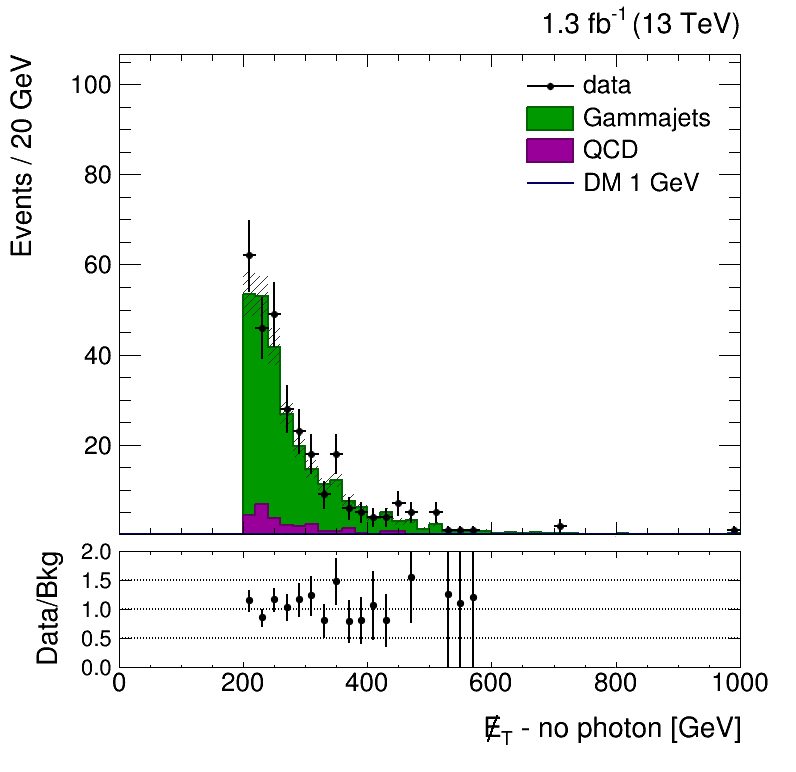
\includegraphics[width=0.48\textwidth]{figures/hPFMETnopholinear_CRzjets.png}
  \caption{The $\met$ distribution in the $\Zjets$ control region with photons for the hadronic channel.}
  \label{fig:incl_hadronic_pho_fmet}
\end{figure}

\subsubsection{Control region for QCD}
\label{subsubsec:bkg_hadronic_qcd}

To obtain a control region enriched in QCD, consider events with no $\Bot$-tagged jets and $\min_{i=1,\ldots,6}\Delta\phi\left(j_i,\,\met\right)<1$. Typically, MC samples for QCD are very statistically limited so the purpose of the control region is to verify that QCD is negligible by looking at the level of data/MC agreement as $\min_{i=1,\ldots,6}\Delta\phi\left(j_i,\,\met\right)$ approaches $1$. If the agreement is good, then it can be concluded that the QCD contribution is negligible. The $\Delta\phi$ distribution in this region is shown in Fig.~\ref{fig:incl_hadronic_qcd_dphijetmet}.

\begin{figure}[htbp]
  \centering
  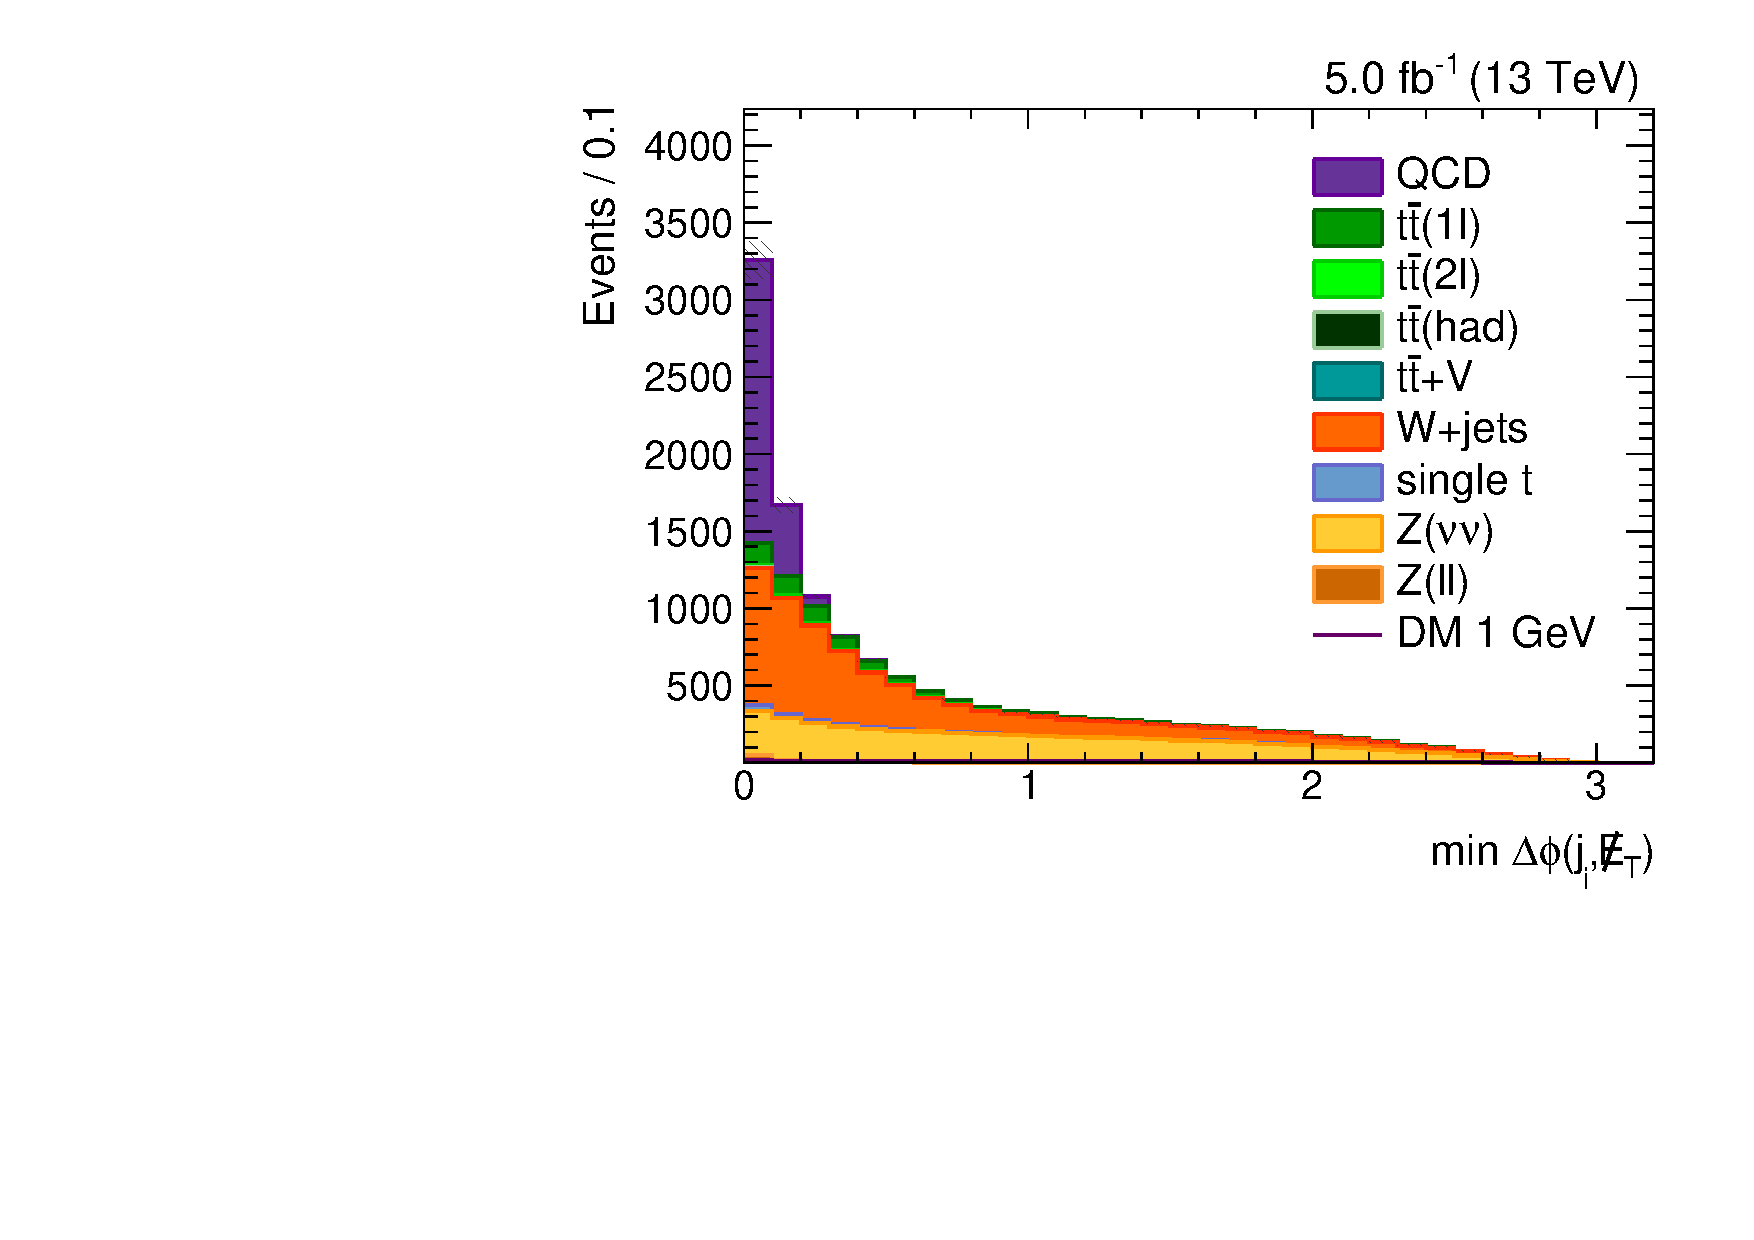
\includegraphics[width=0.48\textwidth]{figures/hadronic-incl-qcd-dphijetmet.pdf}
  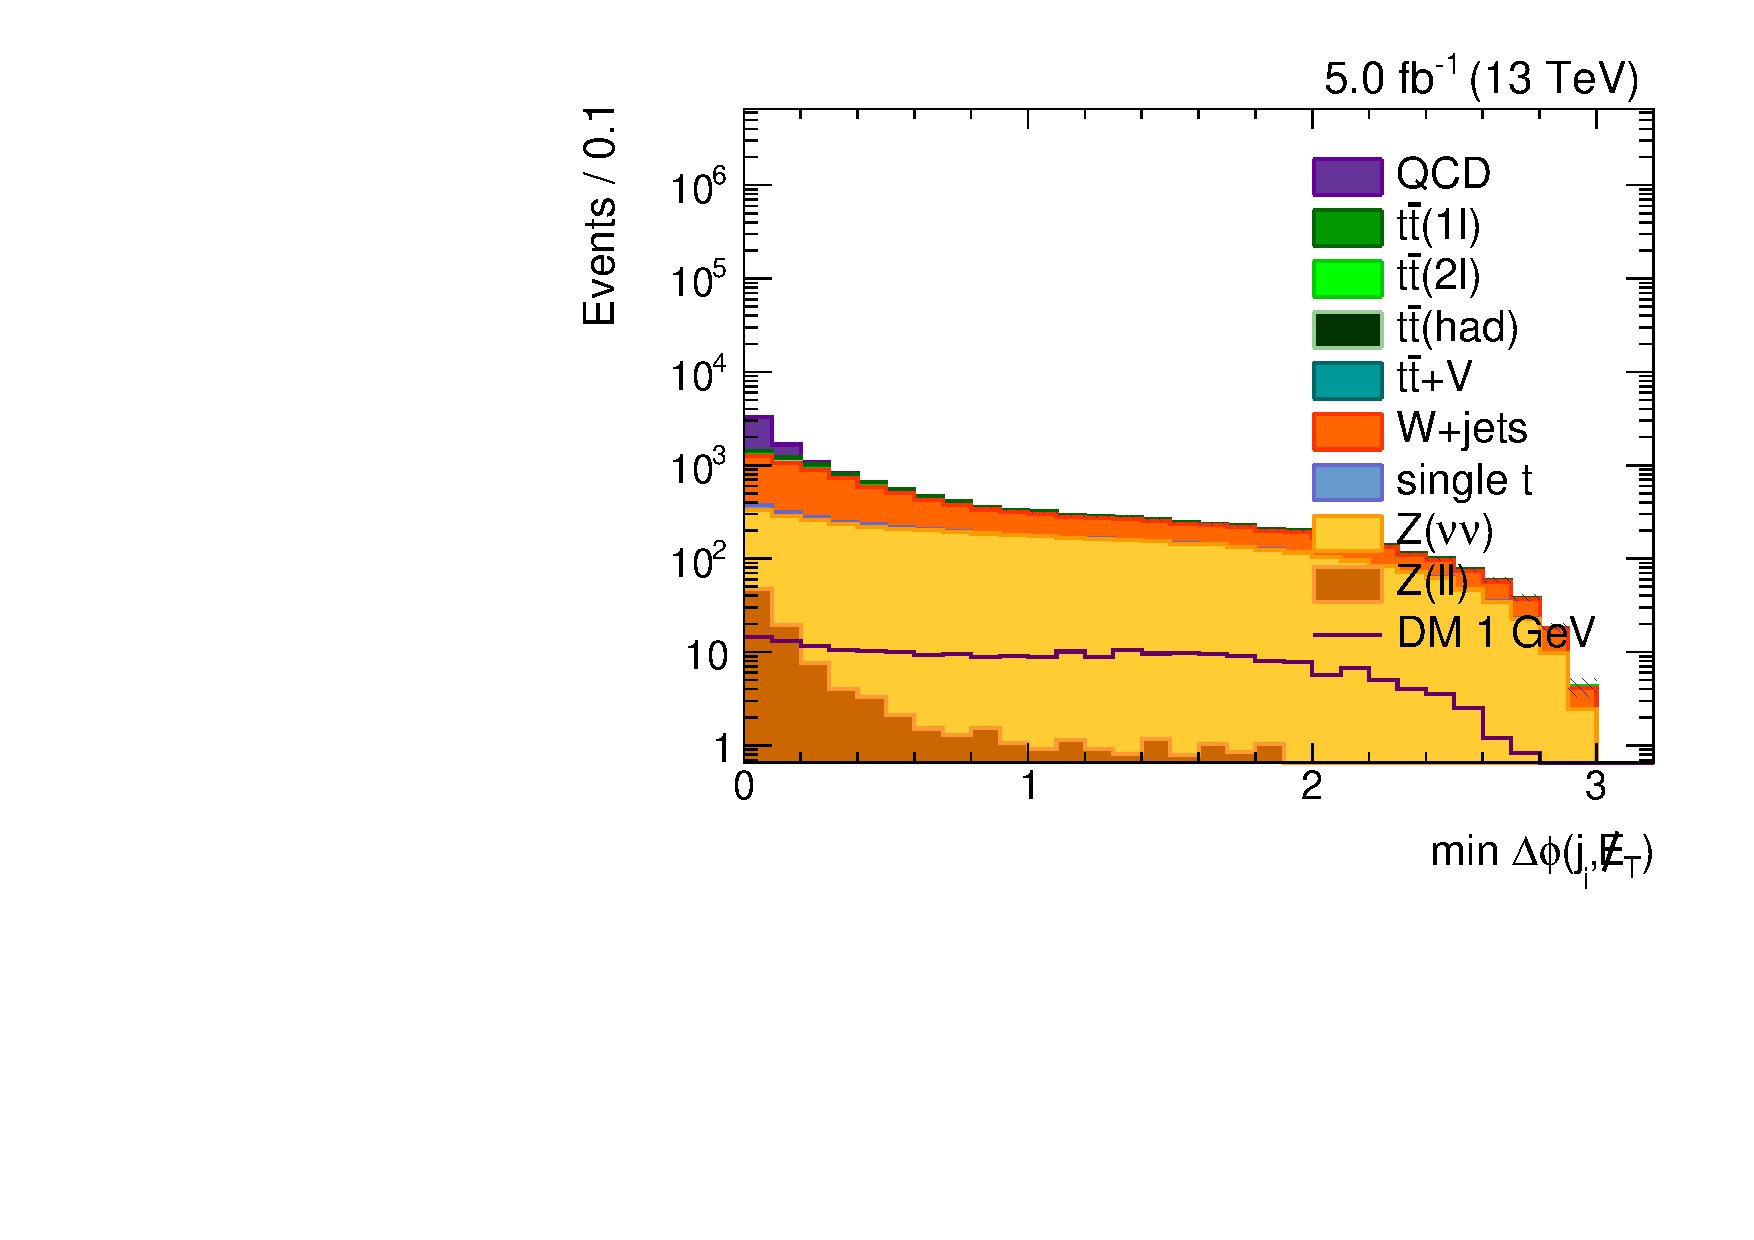
\includegraphics[width=0.48\textwidth]{figures/hadronic-incl-qcd-dphijetmetlog.pdf}
  \caption{The $\min_{i=1,\ldots,6}\Delta\phi\left(j_i,\,\met\right)$ distribution in the QCD control region for the hadronic channel.}
  \label{fig:incl_hadronic_qcd_dphijetmet}
\end{figure}

\subsection{Backgrounds: Semileptonic channel}
\label{subsec:bkg_semilept}

Control regions for the two major backgrounds, dileptonic $\ttbar$ and $\Wjets$, are described in the following.

\subsubsection{Control region for \texorpdfstring{$\ttbar$}{ttbar}}
\label{subsubsec:bkg_semilept_ttbar}

A control region enriched in dileptonic $\ttbar$ can be obtained by requiring a $ee$, $e\mu$, and $\mu\mu$ dilepton pairs where each lepton passes ``Tight'' selection. The four-momentum of the trailing lepton is subtracted from the event to construct the $\met$ template, and is used to compute all $\met$-related variables: $M_T, M_{T2}^W, \min_{i=1,2}\Delta\phi\left(j_i,\,\met\right)$. All other selection cuts for the semileptonic channel are applied accordingly. The yields are listed in Table~\ref{tab:semilept_bkg_tt2l_yields}. The lepton subtracted $\met$ distributions in the control region for the inclusive selection is shown in Fig.~\ref{fig:incl_semilept_2l_fmet}.

\begin{table}[!ht]
\centering
\begin{tabular}{|c|rr|rr|rr|}
\hline
  Process & \multicolumn{2}{|c|}{Inclusive} & \iffalse \multicolumn{2}{|c|}{Boosted} &\fi \multicolumn{2}{|c|}{Resolved} \\
          & $e$ & $\mu$                     & \iffalse$e$ & $\mu$                   &\fi $e$ & $\mu$ \\
\hline
  \Z\To\Lep\Lep          & $  0.50 \pm 0.13$ & $  0.62 \pm 0.12$  &\iffalse $ 0.19 \pm 0.09$ & $ 0.12 \pm 0.02$  &\fi $  0.38 \pm 0.11$ & $  0.52 \pm 0.11$ \\
  Single \Top            & $ 11.80 \pm 1.46$ & $ 13.35 \pm 1.56$  &\iffalse $ 1.09 \pm 0.45$ & $ 1.64 \pm 0.55$  & \fi$ 11.25 \pm 1.43$ & $ 12.26 \pm 1.49$ \\
  \Wjets                 & $  0.03 \pm 0.03$ & $  0.03 \pm 0.03$  & \iffalse$ 0.03 \pm 0.03$ & $ 0.00 \pm 0.00$  & \fi$  0.03 \pm 0.03$ & $  0.03 \pm 0.03$ \\
  $\ttbar+V$             & $  1.86 \pm 0.16$ & $  1.86 \pm 0.03$  & \iffalse$ 0.62 \pm 0.09$ & $ 0.55 \pm 0.09$  & \fi$  1.52 \pm 0.15$ & $  1.51 \pm 0.15$ \\
  $\ttbar(\mbox{had})$   & $  0.00 \pm 0.00$ & $  0.00 \pm 0.00$  &\iffalse $ 0.00 \pm 0.00$ & $ 0.00 \pm 0.00$  & \fi$  0.00 \pm 0.00$ & $  0.00 \pm 0.00$ \\
  $\ttbar(1\Lep)$        & $  0.16 \pm 0.16$ & $  0.00 \pm 0.00$  &\iffalse $ 0.00 \pm 0.00$ & $ 0.00 \pm 0.00$  & \fi$  0.16 \pm 0.16$ & $  0.00 \pm 0.00$ \\
  $\ttbar(2\Lep)$        & $107.05 \pm 4.18$ & $112.77 \pm 4.29$  &\iffalse $13.73 \pm 1.50$ & $14.71 \pm 1.55$  &\fi $102.80 \pm 4.10$ & $108.35 \pm 4.21$ \\
\hline
  SM expected            & $121.39 \pm 4.44$ & $128.63 \pm 4.57$  &\iffalse $15.65 \pm 1.57$ & $17.01 \pm 1.65$  & \fi$116.13 \pm 4.35$ & $122.68 \pm 4.47$ \\
\hline
  $M_\chi=1\:\GeV$       & $  4.94 \pm 0.45$ & $  6.38 \pm 0.51$  &\iffalse $ 0.16 \pm 0.08$ & $ 0.53 \pm 0.15$  &\fi $  4.81 \pm 0.44$ & $  6.21 \pm 0.51$ \\
\hline
\end{tabular}
\caption{Expected yields for $5\:\ifb$ in the $\ttbar$ control region for the semileptonic channel.}
\label{tab:semilept_bkg_tt2l_yields}
\end{table}

\begin{figure}[htbp]
  \centering
  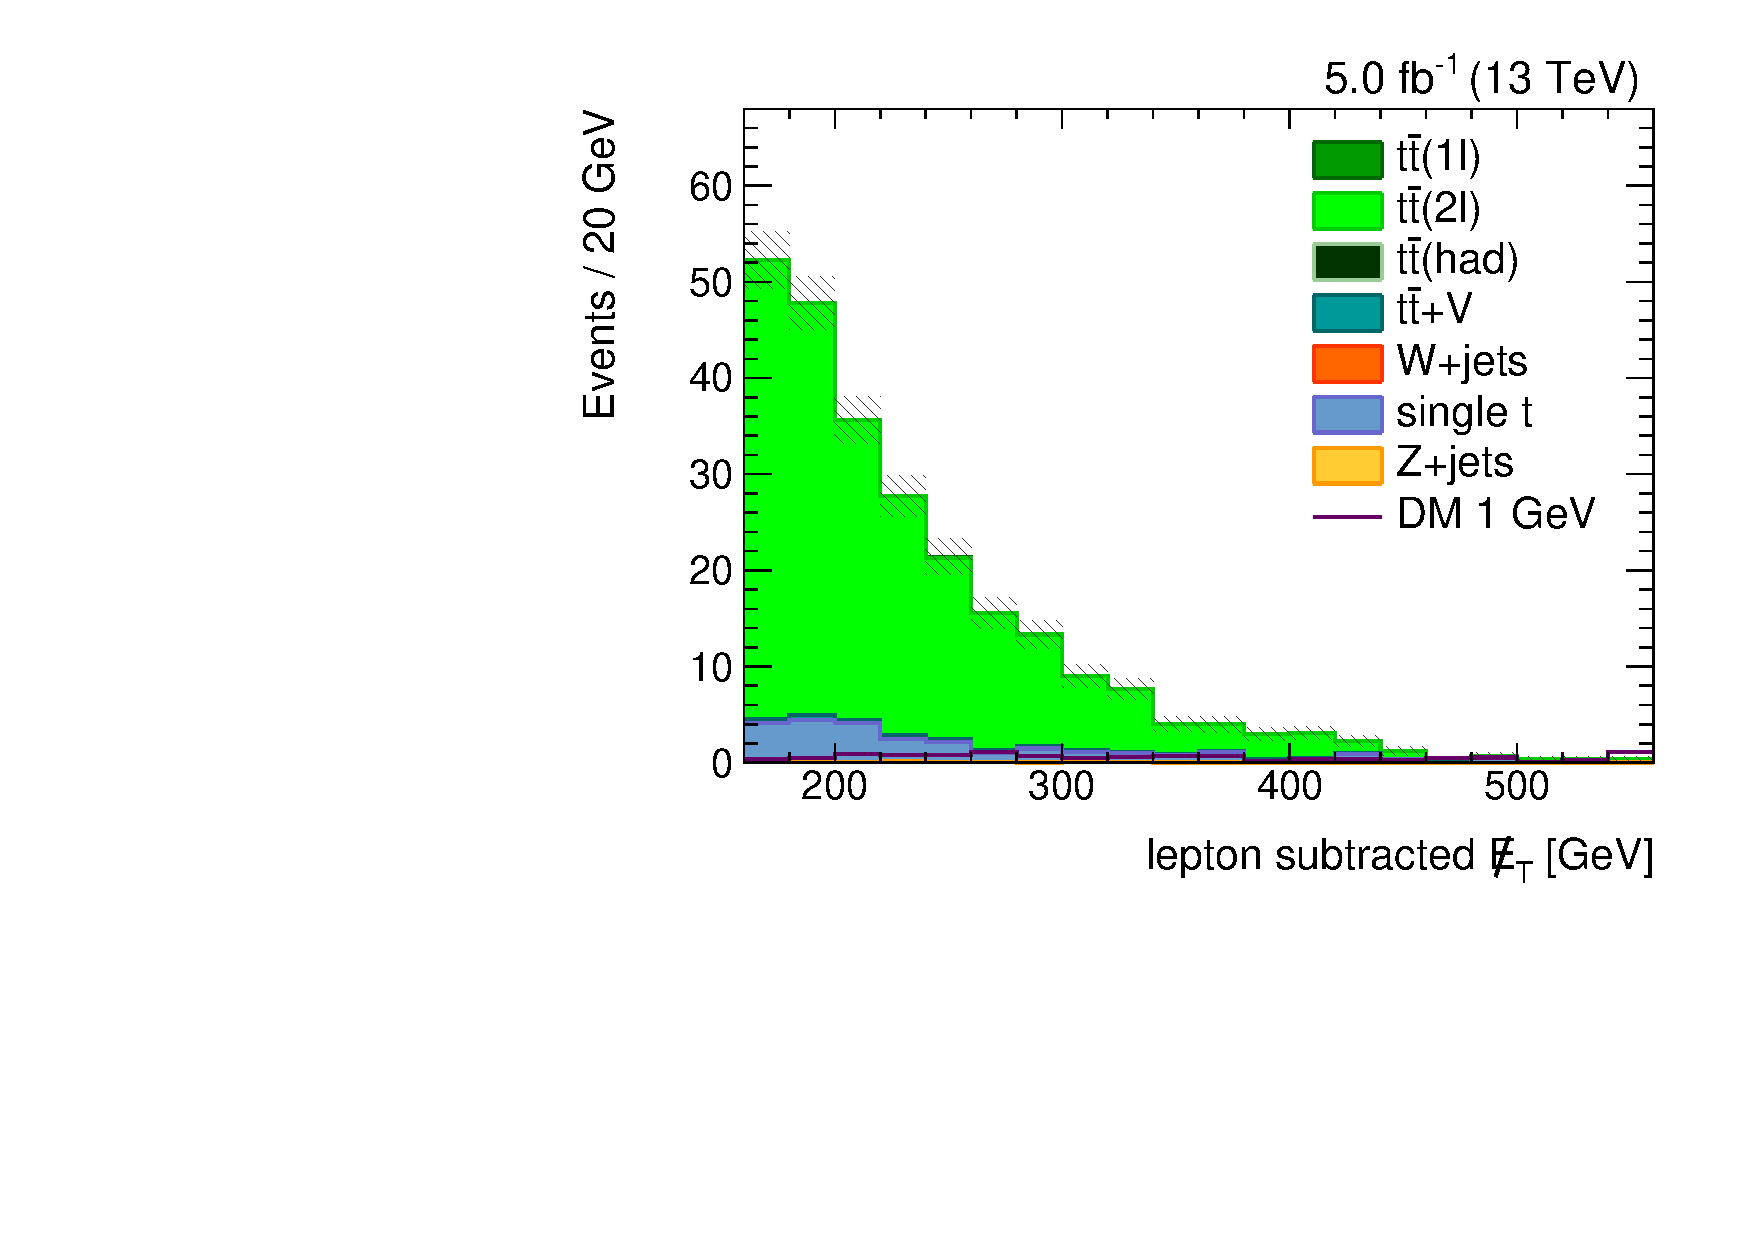
\includegraphics[width=0.48\textwidth]{figures/semilept-incl-2l-fmet_l.pdf}
  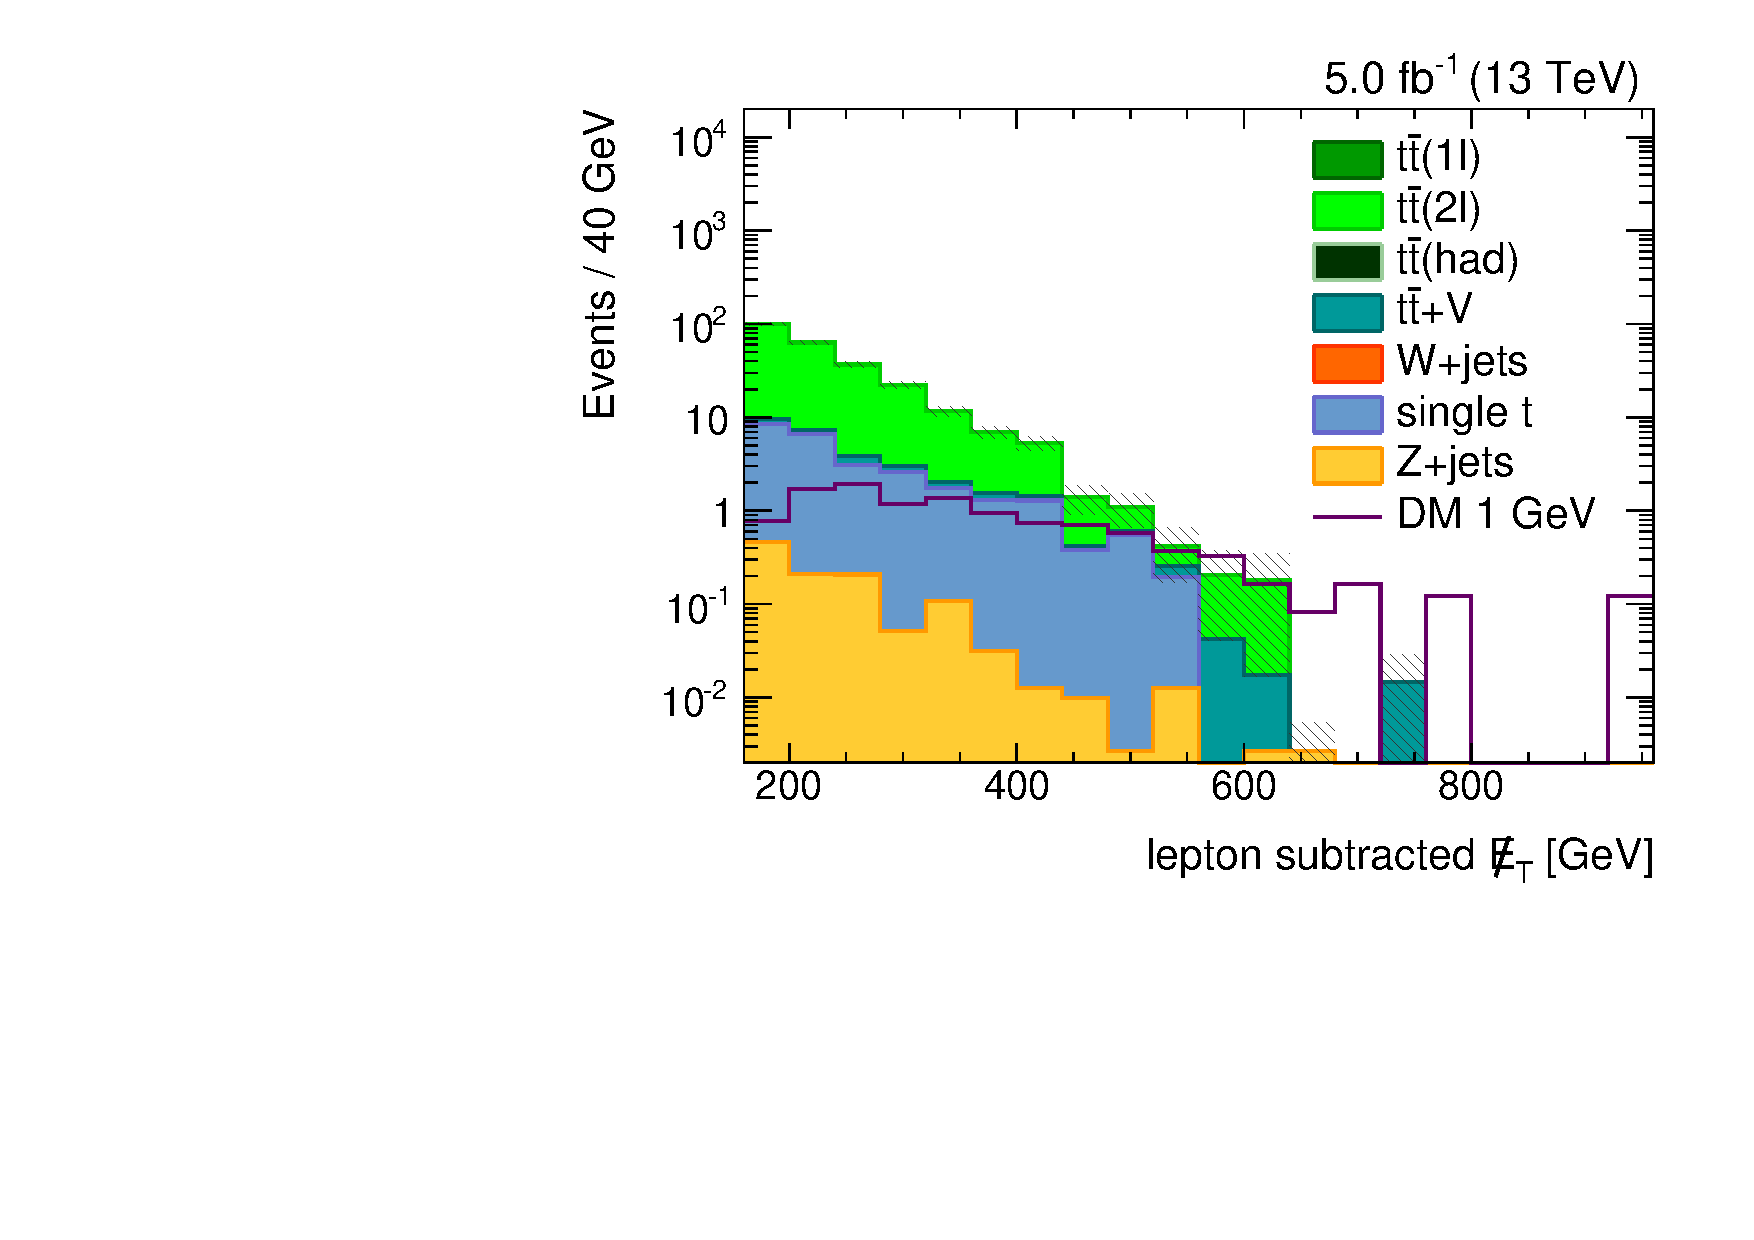
\includegraphics[width=0.48\textwidth]{figures/semilept-incl-2l-fmetlog_l.pdf}
  \caption{The $\met$ distribution in the $\ttbar$ control region for the semileptonic channel.}
  \label{fig:incl_semilept_2l_fmet}
\end{figure}

\subsubsection{Control region for \texorpdfstring{$\Wjets$}{Wjets}}
\label{subsubsec:bkg_semilept_wjets}

By requiring no $\Bot$-tagged jets in the event and keeping all other cuts the same, a sample enriched in $\Wjets$  can be obtained. \iffalse For the categories with boosted top tags, the subjet $\Bot$-tag requirements are dropped. \fi The yields are listed in Table~\ref{tab:semilept_bkg_wjets_yields}. The $\met$ distributions in the control region for the inclusive selection is shown in Fig.~\ref{fig:incl_semilept_0b_met}.

\begin{table}[!ht]
\centering
\begin{tabular}{|c|rr|rr|rr|}
\hline
  Process & \multicolumn{2}{|c|}{Inclusive} &\iffalse \multicolumn{2}{|c|}{Boosted} &\fi \multicolumn{2}{|c|}{Resolved} \\
          & $e$ & $\mu$                     & \iffalse$e$ & $\mu$                   &\fi $e$ & $\mu$ \\
\hline
  \Z\To\Lep\Lep          & $ 0.40 \pm 0.26$ & $ 0.51 \pm 0.11$  &\iffalse $ 0.12 \pm 0.03$ & $ 0.53 \pm 0.14$  & \fi$ 0.38 \pm 0.26$ & $ 0.43 \pm 0.11$ \\
  Single \Top            & $ 1.33 \pm 0.49$ & $ 1.52 \pm 0.52$  & \iffalse$ 0.55 \pm 0.32$ & $ 0.78 \pm 0.37$  &\fi $ 1.15 \pm 0.45$ & $ 1.28 \pm 0.48$ \\
  \Wjets                 & $46.58 \pm 4.47$ & $57.74 \pm 5.59$  & \iffalse$20.18 \pm 2.60$ & $24.80 \pm 2.98$  &\fi $40.75 \pm 4.33$ & $50.33 \pm 5.44$ \\
  $\ttbar+V$             & $ 0.44 \pm 0.08$ & $ 0.64 \pm 0.09$  & \iffalse$ 0.56 \pm 0.09$ & $ 0.67 \pm 0.10$  & \fi$ 0.31 \pm 0.07$ & $ 0.51 \pm 0.08$ \\
  $\ttbar(\mbox{had})$   & $ 0.00 \pm 0.00$ & $ 0.00 \pm 0.00$  & \iffalse$ 0.00 \pm 0.00$ & $ 0.00 \pm 0.00$  & \fi$ 0.00 \pm 0.00$ & $ 0.00 \pm 0.00$ \\
  $\ttbar(1\Lep)$        & $ 0.16 \pm 0.16$ & $ 0.16 \pm 0.16$  & \iffalse$ 0.33 \pm 0.23$ & $ 1.14 \pm 0.43$  & \fi$ 8.83 \pm 1.20$ & $10.79 \pm 1.33$ \\
  $\ttbar(2\Lep)$        & $ 9.97 \pm 1.28$ & $12.09 \pm 1.41$  &\iffalse $ 8.17 \pm 1.16$ & $ 9.15 \pm 1.22$  & \fi$ 0.16 \pm 0.16$ & $ 0.16 \pm 0.16$ \\
\hline
  SM expected            & $58.88 \pm 4.69$ & $72.67 \pm 5.79$  &\iffalse $29.89 \pm 2.87$ & $37.07 \pm 3.27$  & \fi$51.57 \pm 4.53$ & $63.50 \pm 5.63$ \\
\hline
  $M_\chi=1\:\GeV$       & $10.24 \pm 0.65$ & $12.01 \pm 0.70$  & \iffalse$ 6.62 \pm 0.52$ & $ 8.35 \pm 0.59$  &\fi $ 7.69 \pm 0.56$ & $ 8.43 \pm 0.59$ \\
\hline
\end{tabular}
\caption{Expected yields for $5\:\ifb$ in the $\Wjets$ control region for the semileptonic channel.}
\label{tab:semilept_bkg_wjets_yields}
\end{table}

\begin{figure}[htbp]
  \centering
  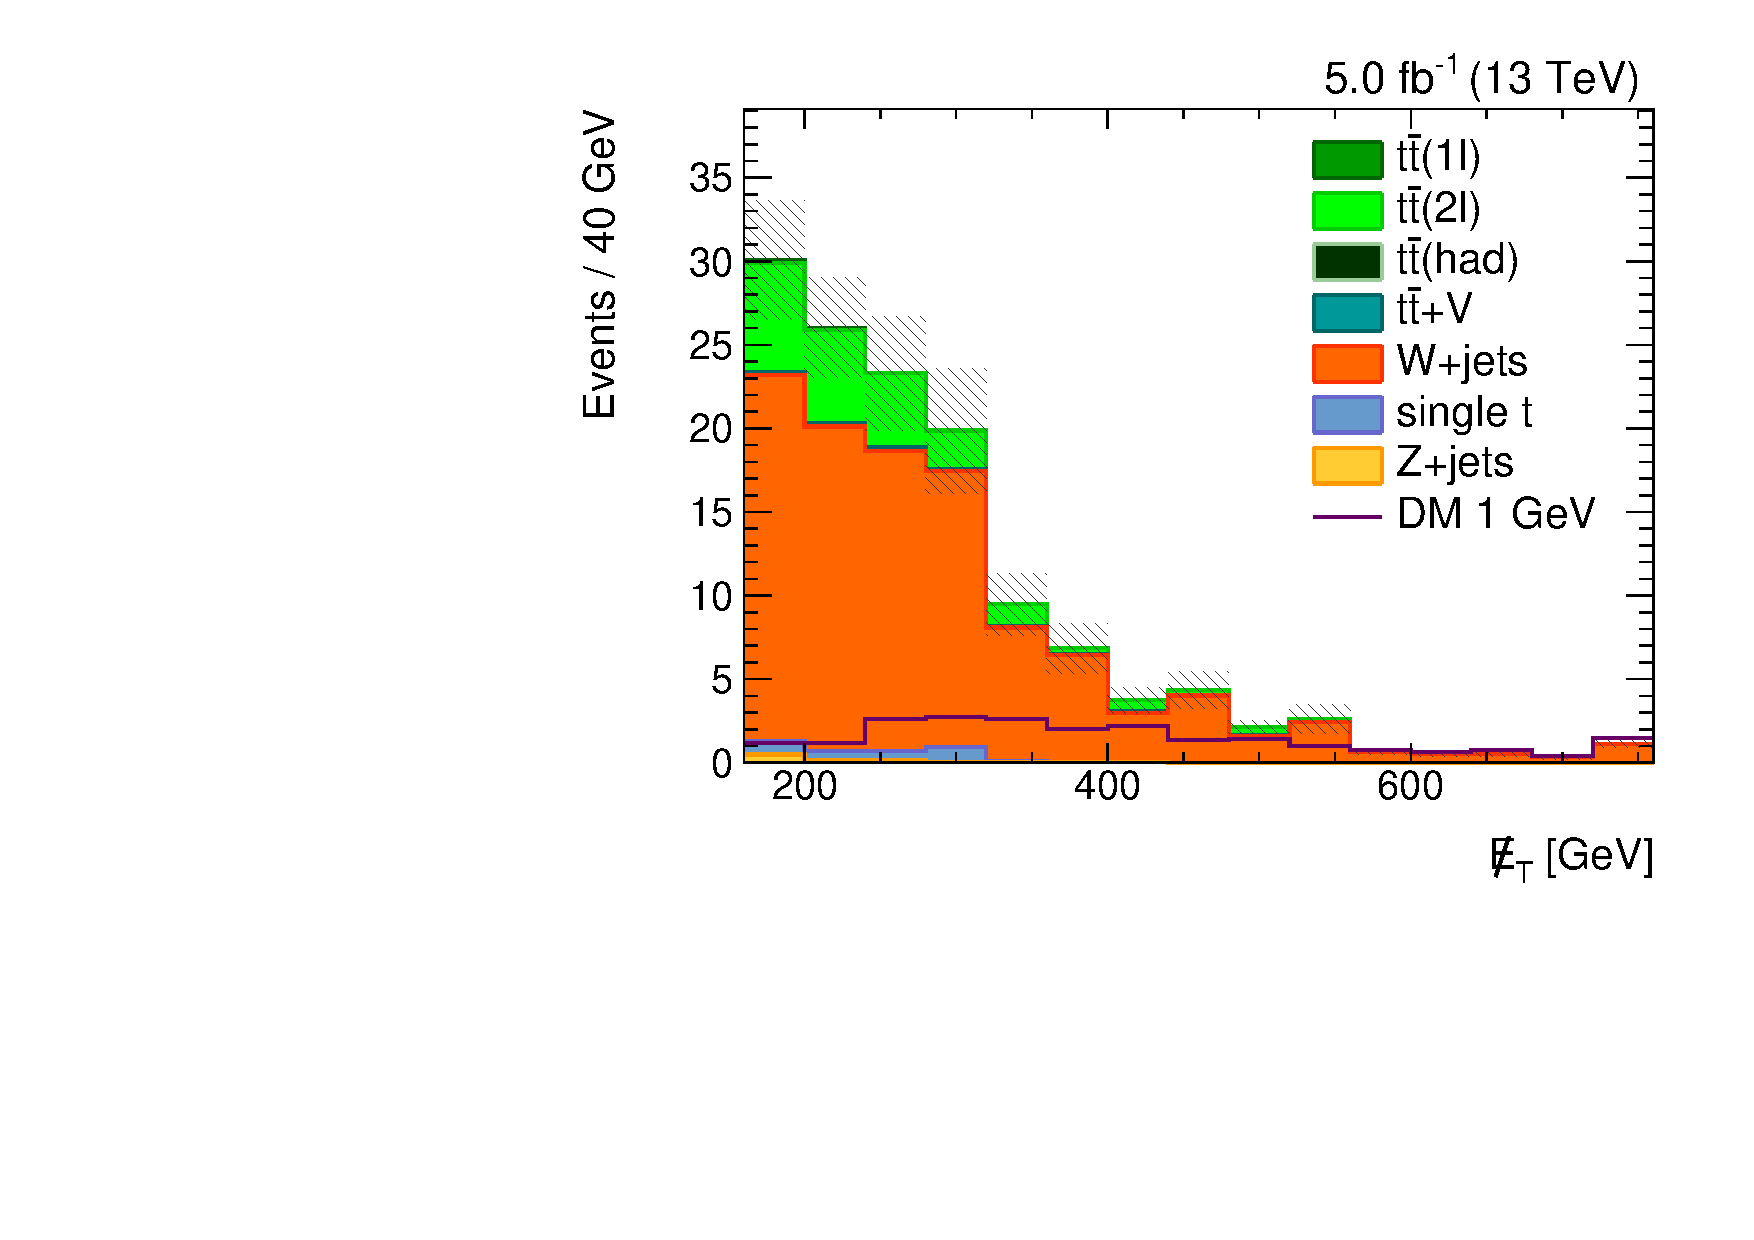
\includegraphics[width=0.48\textwidth]{figures/semilept-incl-0b-met_l.pdf}
  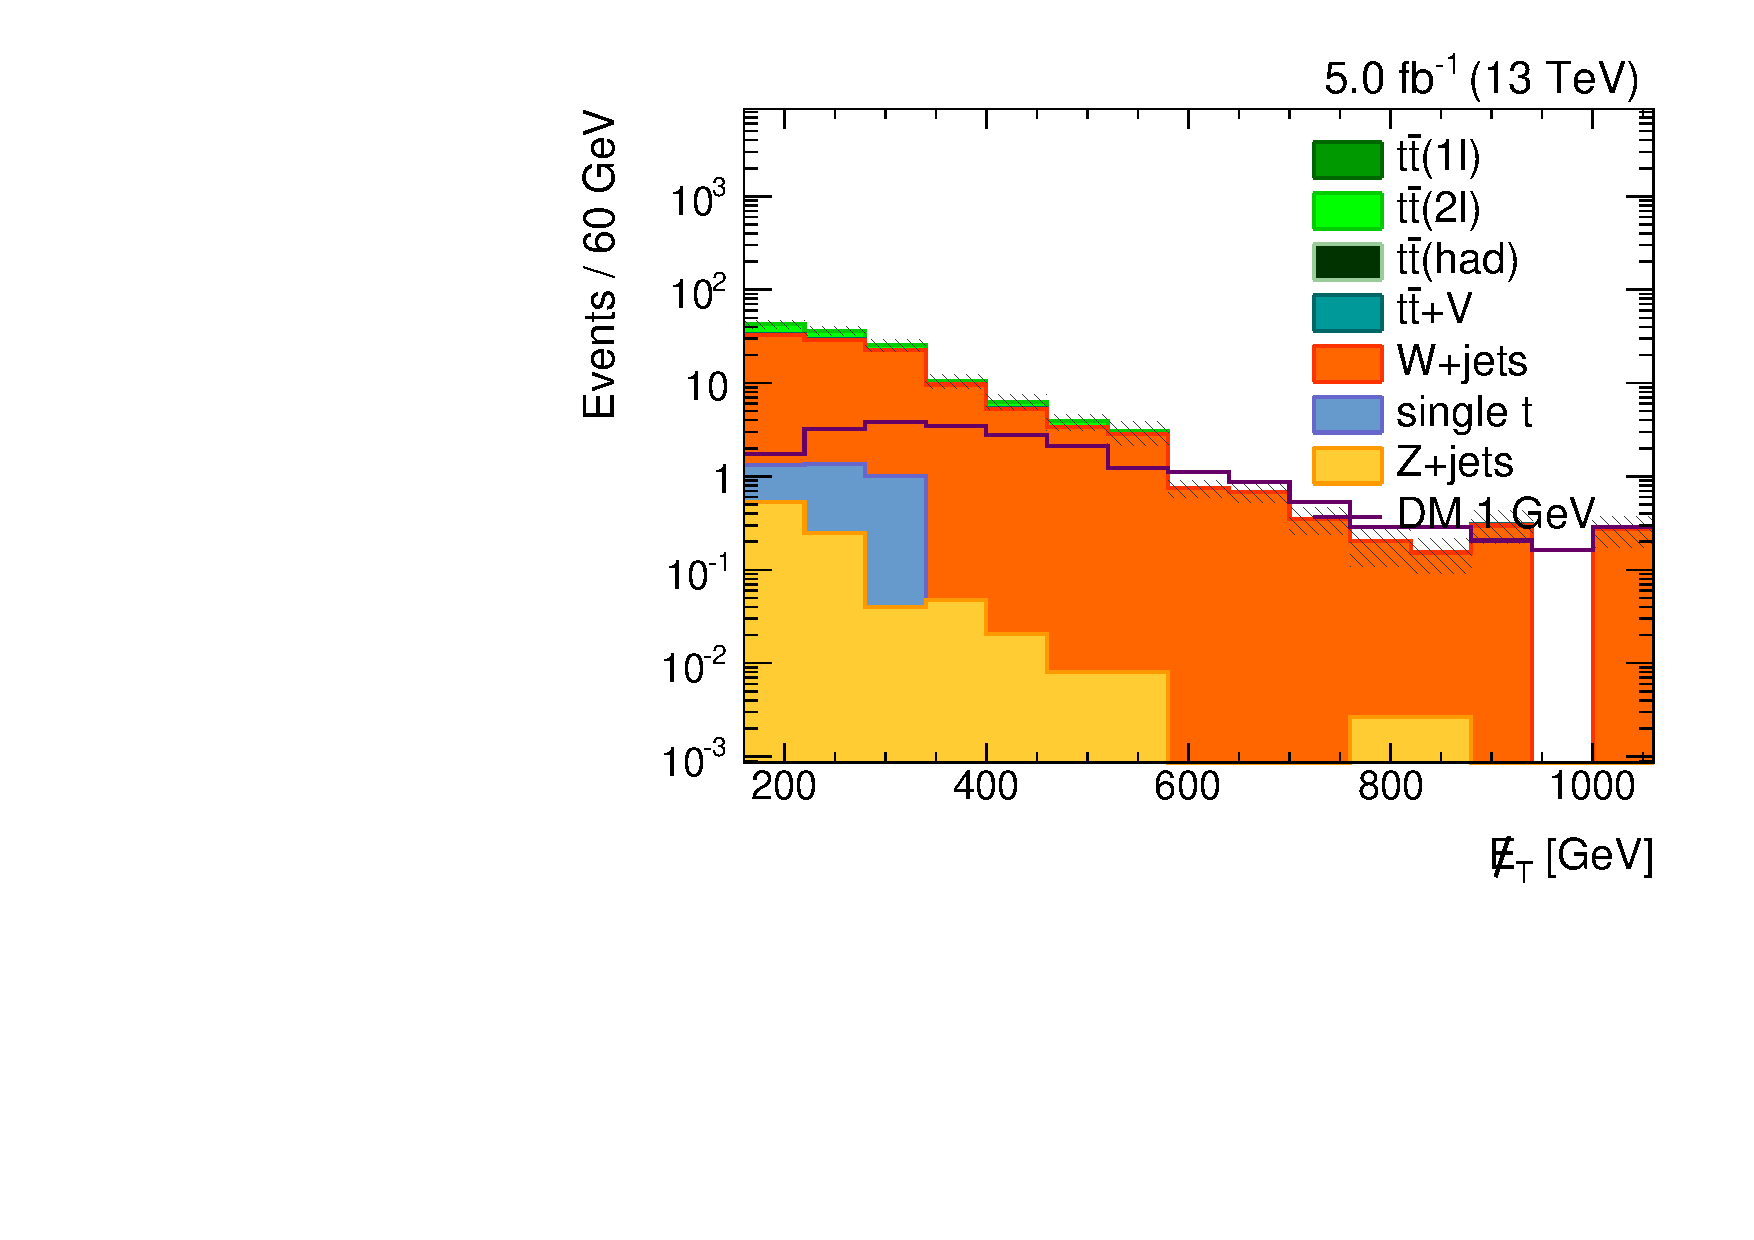
\includegraphics[width=0.48\textwidth]{figures/semilept-incl-0b-metlog_l.pdf}
  \caption{The $\met$ distribution in the $\Wjets$ control region for the semileptonic channel.}
  \label{fig:incl_semilept_0b_met}
\end{figure}

